
%% bare_jrnl_comsoc.tex
%% V1.4b
%% 2015/08/26
%% by Michael Shell
%% see http://www.michaelshell.org/
%% for current contact information.
%%
%% This is a skeleton file demonstrating the use of IEEEtran.cls
%% (requires IEEEtran.cls version 1.8b or later) with an IEEE
%% Communications Society journal paper.
%%
%% Support sites:
%% http://www.michaelshell.org/tex/ieeetran/
%% http://www.ctan.org/pkg/ieeetran
%% and
%% http://www.ieee.org/

%%*************************************************************************
%% Legal Notice:
%% This code is offered as-is without any warranty either expressed or
%% implied; without even the implied warranty of MERCHANTABILITY or
%% FITNESS FOR A PARTICULAR PURPOSE! 
%% User assumes all risk.
%% In no event shall the IEEE or any contributor to this code be liable for
%% any damages or losses, including, but not limited to, incidental,
%% consequential, or any other damages, resulting from the use or misuse
%% of any information contained here.
%%
%% All comments are the opinions of their respective authors and are not
%% necessarily endorsed by the IEEE.
%%
%% This work is distributed under the LaTeX Project Public License (LPPL)
%% ( http://www.latex-project.org/ ) version 1.3, and may be freely used,
%% distributed and modified. A copy of the LPPL, version 1.3, is included
%% in the base LaTeX documentation of all distributions of LaTeX released
%% 2003/12/01 or later.
%% Retain all contribution notices and credits.
%% ** Modified files should be clearly indicated as such, including  **
%% ** renaming them and changing author support contact information. **
%%*************************************************************************


% *** Authors should verify (and, if needed, correct) their LaTeX system  ***
% *** with the testflow diagnostic prior to trusting their LaTeX platform ***
% *** with production work. The IEEE's font choices and paper sizes can   ***
% *** trigger bugs that do not appear when using other class files.       ***                          ***
% The testflow support page is at:
% http://www.michaelshell.org/tex/testflow/



\documentclass[journal,comsoc]{IEEEtran}
%
% If IEEEtran.cls has not been installed into the LaTeX system files,
% manually specify the path to it like:
% \documentclass[journal,comsoc]{../sty/IEEEtran}


\usepackage[T1]{fontenc}% optional T1 font encoding


% Some very useful LaTeX packages include:
% (uncomment the ones you want to load)


% *** MISC UTILITY PACKAGES ***
%
%\usepackage{ifpdf}
% Heiko Oberdiek's ifpdf.sty is very useful if you need conditional
% compilation based on whether the output is pdf or dvi.
% usage:
% \ifpdf
%   % pdf code
% \else
%   % dvi code
% \fi
% The latest version of ifpdf.sty can be obtained from:
% http://www.ctan.org/pkg/ifpdf
% Also, note that IEEEtran.cls V1.7 and later provides a builtin
% \ifCLASSINFOpdf conditional that works the same way.
% When switching from latex to pdflatex and vice-versa, the compiler may
% have to be run twice to clear warning/error messages.






% *** CITATION PACKAGES ***
%
\usepackage{cite}
% cite.sty was written by Donald Arseneau
% V1.6 and later of IEEEtran pre-defines the format of the cite.sty package
% \cite{} output to follow that of the IEEE. Loading the cite package will
% result in citation numbers being automatically sorted and properly
% "compressed/ranged". e.g., [1], [9], [2], [7], [5], [6] without using
% cite.sty will become [1], [2], [5]--[7], [9] using cite.sty. cite.sty's
% \cite will automatically add leading space, if needed. Use cite.sty's
% noadjust option (cite.sty V3.8 and later) if you want to turn this off
% such as if a citation ever needs to be enclosed in parenthesis.
% cite.sty is already installed on most LaTeX systems. Be sure and use
% version 5.0 (2009-03-20) and later if using hyperref.sty.
% The latest version can be obtained at:
% http://www.ctan.org/pkg/cite
% The documentation is contained in the cite.sty file itself.






% *** GRAPHICS RELATED PACKAGES ***
%
\ifCLASSINFOpdf
   \usepackage[pdftex]{graphicx}
  % declare the path(s) where your graphic files are
  % \graphicspath{{../pdf/}{../jpeg/}}
  % and their extensions so you won't have to specify these with
  % every instance of \includegraphics
  % \DeclareGraphicsExtensions{.pdf,.jpeg,.png}
\else
  % or other class option (dvipsone, dvipdf, if not using dvips). graphicx
  % will default to the driver specified in the system graphics.cfg if no
  % driver is specified.
  % \usepackage[dvips]{graphicx}
  % declare the path(s) where your graphic files are
  % \graphicspath{{../eps/}}
  % and their extensions so you won't have to specify these with
  % every instance of \includegraphics
  % \DeclareGraphicsExtensions{.eps}
\fi
% graphicx was written by David Carlisle and Sebastian Rahtz. It is
% required if you want graphics, photos, etc. graphicx.sty is already
% installed on most LaTeX systems. The latest version and documentation
% can be obtained at: 
% http://www.ctan.org/pkg/graphicx
% Another good source of documentation is "Using Imported Graphics in
% LaTeX2e" by Keith Reckdahl which can be found at:
% http://www.ctan.org/pkg/epslatex
%
% latex, and pdflatex in dvi mode, support graphics in encapsulated
% postscript (.eps) format. pdflatex in pdf mode supports graphics
% in .pdf, .jpeg, .png and .mps (metapost) formats. Users should ensure
% that all non-photo figures use a vector format (.eps, .pdf, .mps) and
% not a bitmapped formats (.jpeg, .png). The IEEE frowns on bitmapped formats
% which can result in "jaggedy"/blurry rendering of lines and letters as
% well as large increases in file sizes.
%
% You can find documentation about the pdfTeX application at:
% http://www.tug.org/applications/pdftex





% *** MATH PACKAGES ***
%
\usepackage{amsmath}
% A popular package from the American Mathematical Society that provides
% many useful and powerful commands for dealing with mathematics.
% Do NOT use the amsbsy package under comsoc mode as that feature is
% already built into the Times Math font (newtxmath, mathtime, etc.).
% 
% Also, note that the amsmath package sets \interdisplaylinepenalty to 10000
% thus preventing page breaks from occurring within multiline equations. Use:
\interdisplaylinepenalty=2500
% after loading amsmath to restore such page breaks as IEEEtran.cls normally
% does. amsmath.sty is already installed on most LaTeX systems. The latest
% version and documentation can be obtained at:
% http://www.ctan.org/pkg/amsmath


% Select a Times math font under comsoc mode or else one will automatically
% be selected for you at the document start. This is required as Communications
% Society journals use a Times, not Computer Modern, math font.
\usepackage[cmintegrals]{newtxmath}
% The freely available newtxmath package was written by Michael Sharpe and
% provides a feature rich Times math font. The cmintegrals option, which is
% the default under IEEEtran, is needed to get the correct style integral
% symbols used in Communications Society journals. Version 1.451, July 28,
% 2015 or later is recommended. Also, do *not* load the newtxtext.sty package
% as doing so would alter the main text font.
% http://www.ctan.org/pkg/newtx
%
% Alternatively, you can use the MathTime commercial fonts if you have them
% installed on your system:
%\usepackage{mtpro2}
%\usepackage{mt11p}
%\usepackage{mathtime}


%\usepackage{bm}
% The bm.sty package was written by David Carlisle and Frank Mittelbach.
% This package provides a \bm{} to produce bold math symbols.
% http://www.ctan.org/pkg/bm





% *** SPECIALIZED LIST PACKAGES ***
%
%\usepackage{algorithmic}
% algorithmic.sty was written by Peter Williams and Rogerio Brito.
% This package provides an algorithmic environment fo describing algorithms.
% You can use the algorithmic environment in-text or within a figure
% environment to provide for a floating algorithm. Do NOT use the algorithm
% floating environment provided by algorithm.sty (by the same authors) or
% algorithm2e.sty (by Christophe Fiorio) as the IEEE does not use dedicated
% algorithm float types and packages that provide these will not provide
% correct IEEE style captions. The latest version and documentation of
% algorithmic.sty can be obtained at:
% http://www.ctan.org/pkg/algorithms
% Also of interest may be the (relatively newer and more customizable)
% algorithmicx.sty package by Szasz Janos:
% http://www.ctan.org/pkg/algorithmicx




% *** ALIGNMENT PACKAGES ***
%
%\usepackage{array}
% Frank Mittelbach's and David Carlisle's array.sty patches and improves
% the standard LaTeX2e array and tabular environments to provide better
% appearance and additional user controls. As the default LaTeX2e table
% generation code is lacking to the point of almost being broken with
% respect to the quality of the end results, all users are strongly
% advised to use an enhanced (at the very least that provided by array.sty)
% set of table tools. array.sty is already installed on most systems. The
% latest version and documentation can be obtained at:
% http://www.ctan.org/pkg/array


% IEEEtran contains the IEEEeqnarray family of commands that can be used to
% generate multiline equations as well as matrices, tables, etc., of high
% quality.




% *** SUBFIGURE PACKAGES ***
%\ifCLASSOPTIONcompsoc
%  \usepackage[caption=false,font=normalsize,labelfont=sf,textfont=sf]{subfig}
%\else
%  \usepackage[caption=false,font=footnotesize]{subfig}
%\fi
% subfig.sty, written by Steven Douglas Cochran, is the modern replacement
% for subfigure.sty, the latter of which is no longer maintained and is
% incompatible with some LaTeX packages including fixltx2e. However,
% subfig.sty requires and automatically loads Axel Sommerfeldt's caption.sty
% which will override IEEEtran.cls' handling of captions and this will result
% in non-IEEE style figure/table captions. To prevent this problem, be sure
% and invoke subfig.sty's "caption=false" package option (available since
% subfig.sty version 1.3, 2005/06/28) as this is will preserve IEEEtran.cls
% handling of captions.
% Note that the Computer Society format requires a larger sans serif font
% than the serif footnote size font used in traditional IEEE formatting
% and thus the need to invoke different subfig.sty package options depending
% on whether compsoc mode has been enabled.
%
% The latest version and documentation of subfig.sty can be obtained at:
% http://www.ctan.org/pkg/subfig




% *** FLOAT PACKAGES ***
%
%\usepackage{fixltx2e}
% fixltx2e, the successor to the earlier fix2col.sty, was written by
% Frank Mittelbach and David Carlisle. This package corrects a few problems
% in the LaTeX2e kernel, the most notable of which is that in current
% LaTeX2e releases, the ordering of single and double column floats is not
% guaranteed to be preserved. Thus, an unpatched LaTeX2e can allow a
% single column figure to be placed prior to an earlier double column
% figure.
% Be aware that LaTeX2e kernels dated 2015 and later have fixltx2e.sty's
% corrections already built into the system in which case a warning will
% be issued if an attempt is made to load fixltx2e.sty as it is no longer
% needed.
% The latest version and documentation can be found at:
% http://www.ctan.org/pkg/fixltx2e


%\usepackage{stfloats}
% stfloats.sty was written by Sigitas Tolusis. This package gives LaTeX2e
% the ability to do double column floats at the bottom of the page as well
% as the top. (e.g., "\begin{figure*}[!b]" is not normally possible in
% LaTeX2e). It also provides a command:
%\fnbelowfloat
% to enable the placement of footnotes below bottom floats (the standard
% LaTeX2e kernel puts them above bottom floats). This is an invasive package
% which rewrites many portions of the LaTeX2e float routines. It may not work
% with other packages that modify the LaTeX2e float routines. The latest
% version and documentation can be obtained at:
% http://www.ctan.org/pkg/stfloats
% Do not use the stfloats baselinefloat ability as the IEEE does not allow
% \baselineskip to stretch. Authors submitting work to the IEEE should note
% that the IEEE rarely uses double column equations and that authors should try
% to avoid such use. Do not be tempted to use the cuted.sty or midfloat.sty
% packages (also by Sigitas Tolusis) as the IEEE does not format its papers in
% such ways.
% Do not attempt to use stfloats with fixltx2e as they are incompatible.
% Instead, use Morten Hogholm'a dblfloatfix which combines the features
% of both fixltx2e and stfloats:
%
% \usepackage{dblfloatfix}
% The latest version can be found at:
% http://www.ctan.org/pkg/dblfloatfix




%\ifCLASSOPTIONcaptionsoff
%  \usepackage[nomarkers]{endfloat}
% \let\MYoriglatexcaption\caption
% \renewcommand{\caption}[2][\relax]{\MYoriglatexcaption[#2]{#2}}
%\fi
% endfloat.sty was written by James Darrell McCauley, Jeff Goldberg and 
% Axel Sommerfeldt. This package may be useful when used in conjunction with 
% IEEEtran.cls'  captionsoff option. Some IEEE journals/societies require that
% submissions have lists of figures/tables at the end of the paper and that
% figures/tables without any captions are placed on a page by themselves at
% the end of the document. If needed, the draftcls IEEEtran class option or
% \CLASSINPUTbaselinestretch interface can be used to increase the line
% spacing as well. Be sure and use the nomarkers option of endfloat to
% prevent endfloat from "marking" where the figures would have been placed
% in the text. The two hack lines of code above are a slight modification of
% that suggested by in the endfloat docs (section 8.4.1) to ensure that
% the full captions always appear in the list of figures/tables - even if
% the user used the short optional argument of \caption[]{}.
% IEEE papers do not typically make use of \caption[]'s optional argument,
% so this should not be an issue. A similar trick can be used to disable
% captions of packages such as subfig.sty that lack options to turn off
% the subcaptions:
% For subfig.sty:
% \let\MYorigsubfloat\subfloat
% \renewcommand{\subfloat}[2][\relax]{\MYorigsubfloat[]{#2}}
% However, the above trick will not work if both optional arguments of
% the \subfloat command are used. Furthermore, there needs to be a
% description of each subfigure *somewhere* and endfloat does not add
% subfigure captions to its list of figures. Thus, the best approach is to
% avoid the use of subfigure captions (many IEEE journals avoid them anyway)
% and instead reference/explain all the subfigures within the main caption.
% The latest version of endfloat.sty and its documentation can obtained at:
% http://www.ctan.org/pkg/endfloat
%
% The IEEEtran \ifCLASSOPTIONcaptionsoff conditional can also be used
% later in the document, say, to conditionally put the References on a 
% page by themselves.




% *** PDF, URL AND HYPERLINK PACKAGES ***
%
%\usepackage{url}
% url.sty was written by Donald Arseneau. It provides better support for
% handling and breaking URLs. url.sty is already installed on most LaTeX
% systems. The latest version and documentation can be obtained at:
% http://www.ctan.org/pkg/url
% Basically, \url{my_url_here}.




% *** Do not adjust lengths that control margins, column widths, etc. ***
% *** Do not use packages that alter fonts (such as pslatex).         ***
% There should be no need to do such things with IEEEtran.cls V1.6 and later.
% (Unless specifically asked to do so by the journal or conference you plan
% to submit to, of course. )


% correct bad hyphenation here
\hyphenation{op-tical net-works semi-conduc-tor}


\begin{document}
\title{A Development Environment for Decomposite MAC Description Language}
\author{Leon Fernandez}
\markboth{ID2205 Final Report}%
{A DE for DMDL}
\maketitle

\begin{abstract}
In order to tackle the ever-increasing demands on wireless capacity and diversity,
Decomposite MAC Description Language (DMDL) has be developed. DMDL is a graphical
programming language that allows the user to intuitively and swiftly describe and
prototype Medium Access Control (MAC) protocols without platform dependence.
In order to embrace the platform independence of DMDL, a web-based Development Environment (DE)
has been built. The DE is thought to act as a front-end in a system that allows a user to
simulate or even implement MAC protocols with frameworks such as LabVIEW and GNU Radio and
platforms such as USRP acting as a back-end. This is arguably an important step towards a
full softwarization of the network stack and can provide much needed flexibility in developing
wireless systems. The DE is mainly used to create and export an XML file that represent the DMDL
description a protocol. The XML file will act as an intermediate file between the DE and existing
frameworks for wireless protocol development.

\end{abstract}

\begin{IEEEkeywords}
Software Defined Radio, Medium Access Control, Graphical Programming.
\end{IEEEkeywords}

\section{Introduction}
\IEEEPARstart{W}{ireless technology} is an essential part of our everyday lives and it is
being adopted literally everywhere. High or low, big or small, wireless technology can
find applications of all kinds. From high performance cellphone base stations to low-cost,
low-energy sensor networks. The diversity of wireless systems is tremendous, to say the least,
and embracing the diversity allows the limited resource that is the Electromagnetic EM spectrum to
be used more efficiently.

The Software Defined Radio (SDR)~\cite{sdr} is a reconfigurable transceiver that can be programmed
to the developer's liking entirely by software. Within the diverse field of wireless research,
it is an essential tool for prototyping and developing the protocols and systems of tomorrow.

The OSI model~\cite{osi} paints a rough picture that provides a basic understanding of
how a networking stack is implemented. It consists of seven layers that each contain different
functionalities that together realize a communication between two networking devices. The bottom
two layers, the Physical (PHY) and Data Link (DL) layers, have traditionally been implemented
in hardware and the remaining five in software. Software implementations are generally more
flexible and easier to develop, which is desirable within a dynamic field such as wireless
research. Through the SDR, the PHY layer can can be be implemented in software as well.

Before a fully softwarized network stack can be realized, a framework for defining DL functionality
is needed. An important step towards that is the softwarization of the DL sublayer
called Medium Access Control (MAC), which provides the functionality of coordination among nodes
in order to keep interferance within a wireless system down. For this,
Decomposite MAC Description Language (DMDL)~\cite{dmdl} has been developed.

By providing a web-based front-end for a DMDL Development Environment (DE) the accessibility
and platform-independence of DMDL can be boosted. Following trends such as
Platform as a Service (PaaS) or Hardware as a Service (HaaS), this project aims to take a first
step towords something that could be regarded as SDR as a Service (SDRaaS). Promoting DMDL in
this was can help achieve a softwarization of the entire network stack, which in turn promotes
diversity so that wireless systems can continue to thrive. 


\section{Related Work}
DMDL is a graphical programming language designed for the purpose of developing and implementing
MAC protocols in a swift and flexible manner whilst being platform-independent. DMDL models
MAC protocols as a Hierarchical Finite State Machine (HFSM)~\cite{hfsm} in which each state is
described by a Synchronous Dataflow Graph (SDF)~\cite{sdf}. This has the advantage over more
traditional models of facilitating cross-layer optimization and providing a better concurrency
model. Additionally, its modular approach to protocol design ensures high code reusability and
flexibility.

The main components of DMDL are blocks, commands and ports. The blocks correspond to actors
in an SDF graph and they perform basic MAC functions such as carrier sensing and framing.
Commands correspond to the tokens in an SDF graph and they are consumed or produced by input
and output ports, respectively. Any given block has a number of mandatory ports which must
be used if the block is to function, and a number of optional ports that the developer may
use if additional functionality of the block is desired.


There are several frameworks for graphically programming SDRs. Arguably, the to most notable
ones are~\cite{labview} and GNU Radio~\cite{gr}, which mainly target the
Universal Software Radio Peripheral (USRP)~\cite{usrp} SDR platform. However, they do not
provide any formal framework for MAC protocol development. Due to the licensing costs of LabVIEW
and the cost of USRP hardware, some developers might see limited use of these frameworks.

By providing a browser-based DE for DMDL that is platform independent, a framework can be provided
to actors otherwise unable to utilize LabVIEW and/or USRP such as small companies or research
groups with limited funds. In a PaaS- or HaaS-like manner, SDR experiment rigs can be provided as a
service, SDRaaS if you will, thereby making an effort to promote swift MAC protocol development and
prototyping.

\section{Method}
As a web-based application, the DE consists solely of JavaScript (JS), HTML 5 and CSS 3 source
code. No web frameworks such as JQuery, React or Angular were used since the developer had no
prior experience with web development and therefore chose to keep everything as simple as possible
as a first iteration of developing the DE. The JS code mainly follows the EcmaScript 5 standard to
ensure compatibility even for older devices and browsers.

\subsection{Code Overview}
Figure~\ref{fig:uml} shows a Universal Modeling Language (UML) diagram for the DE and how the
underlying JS classes interact. The blocks labeled Workspace, BlockEditor and BlockMenu are the
main HTML elements where most of the user interaction is done. The blocks with underlined labels
represent the DMDL components, namely blocks and ports.There is no implementation of the DMDL
command concept, which is why the corresponding blocks have a dashed outline.
\begin{figure}[!t]
\centering
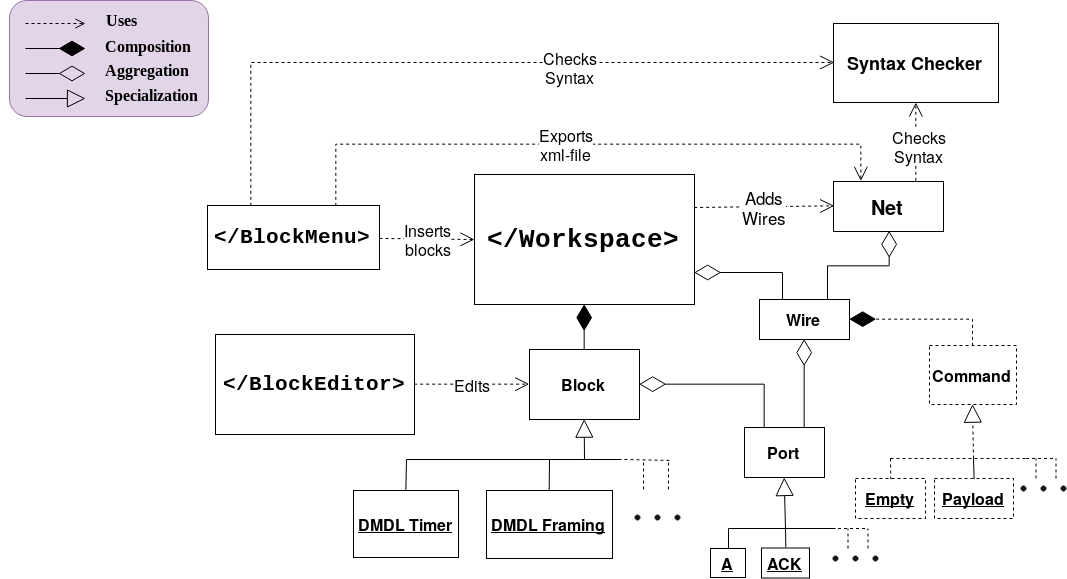
\includegraphics[width=\columnwidth]{dmdl-editor.png}
\caption{A UML overview of the JS code for the DE.}
\label{fig:uml}
\end{figure}

\subsection{DMDL Subclasses}
The structure of the code aims to separate the User Interface UI components and the DMDL components
into different classes in order to achieve a maintainable and easily extendable codebase.
Furthermore, the DMDL classes are kept as minimal as possible in order for easy implementation
of new DMDL blocks or ports, the majority of the functionality (such as being drawn or being
dragged) sits within the corresponding superclasses. Fig.~\ref{fig:timer_src} shows the source code
for the DMDL timer block. It starts by calling the constructor of the block superclass with the
coordinates at which the block is created and a list of ports that are available to the block.
After that is a list of configurable parameters for the block. Lastly, a number of strings
are placed in an associative array where each string represent how a parameter is configurable,
what the options are and what the default value is.
\begin{figure}[!t]
\centering
    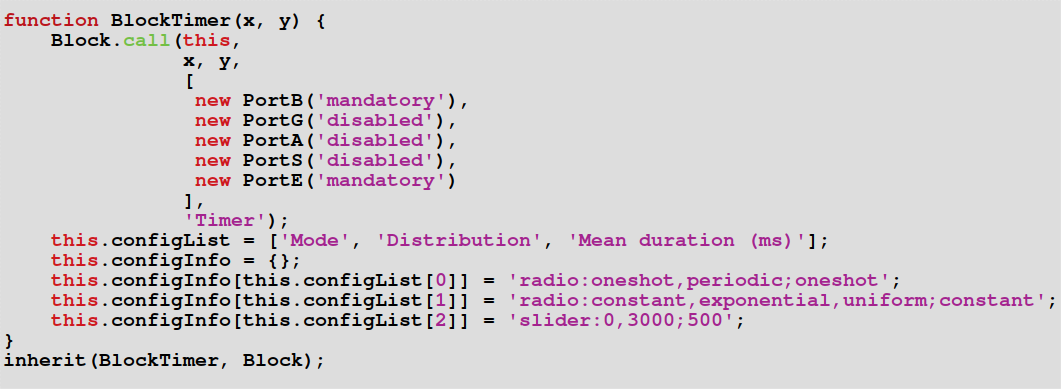
\includegraphics[width=\columnwidth]{timer_src.png}
    \caption{Source code for the Timer class' constructor.}
    \label{fig:timer_src}
\end{figure}

\subsection{Link Between DE and Other Software}
The DE can be used to create an Extensible Markup Language (XML) file that represents the
graph/protocol that the developer has created. The XML file is thought to serve as the main link
between the DE and other tools. XML was chosen since it is widely used to represent software
objects such as graphs or diagrams in professional development tools such as GNU Radio and
LabVIEW. The structure of the XML file was specifically designed for the DE.

The XML file structure is based on the notion of a netlist, which is commonly used within the
electronic design automation industry~\cite{netlist}. Subsection~\ref{sec:xml} discusses the
structure in more detail from an example.

\section{Results and Analysis}
Fig.~\ref{fig:full_editor} shows a screenshot of the Aloha protocol~\cite{aloha} implemented
in the DE. To the left is the block menu, where the user selects which type of block will be
placed. The rightmost element is where the configuration of placed blocks is performed. The
block being configured is chosen by clicking on it, which also marks it with a green rectangle.
The middle element is the main workspace where blocks are dragged around and were wires are
drawn. Wires are drawn by left-clicking on a port and moving the mouse over to another port and
then releasing the button.

The DE has been tested to work in the browsers Firefox 64.0, Chromium 71.0 and Epiphany 3.28.

\begin{figure}[!t]
    \centering
    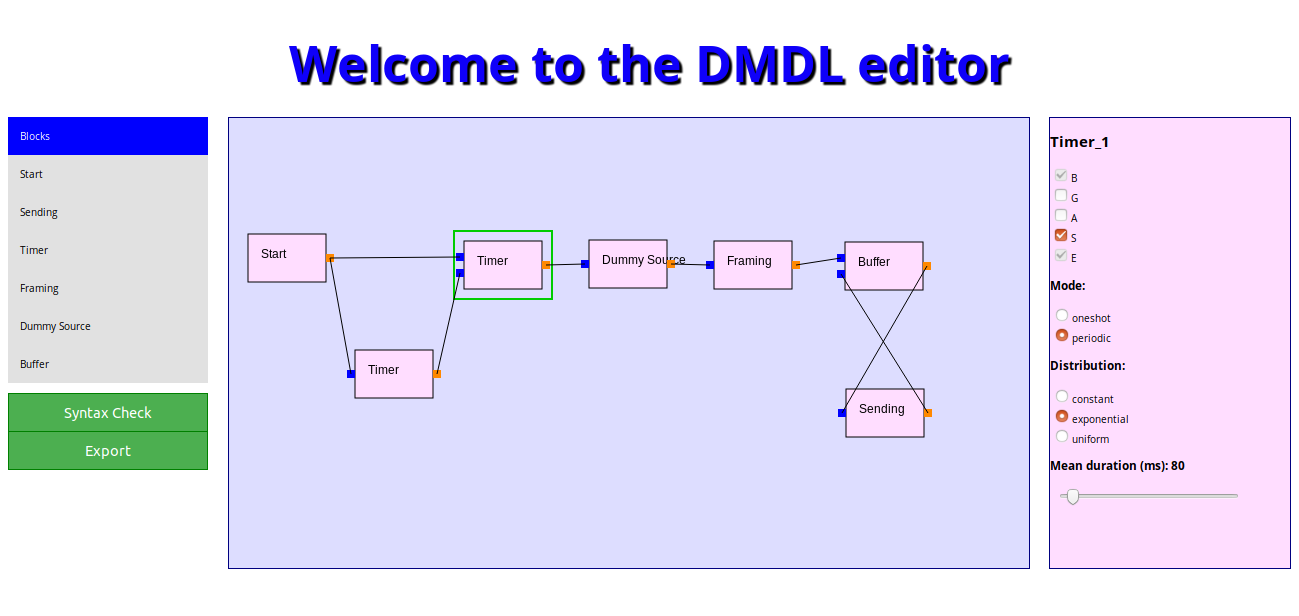
\includegraphics[width=\columnwidth]{full_editor.png}
    \caption{A screenshot of the Aloha protocol~\cite{aloha} implemented in the DE.}
    \label{fig:full_editor}
\end{figure}

\subsection{XML Structure}
\label{sec:xml}
Exporting the drawn graph to an XML file is done in the Net class through a static function.
The net class keeps track of which ports are connected to eachother. If one is able to
travel from one port to another over wires without going through any blocks, the ports
belong to the same net. Fig.~\ref{fig:net} shows the two nets present in a graph representing
a poisson source.

The exported XML mainly consists of a number of block entries, one for each block in the graph.
Fig.~\ref{fig:xml1} and Fig.~\ref{fig:xml2} shows the the XML code for the top right block in
Fig.~\ref{fig:net}. Here follows a rundown of the segments.
\begin{figure}[!t]
    \centering
    \includegraphics[width=\columnwidth]{poisson_block_cfg.pdf}
    \caption{XML code for a timer block entry, part 1.}
    \label{fig:xml1}
\end{figure}
\begin{figure}[!t]
    \centering
    \includegraphics[width=\columnwidth]{poisson_block_port.pdf}
    \caption{XML code for a timer block entry, part 2.}
    \label{fig:xml2}
\end{figure}
\begin{figure}[!t]
    \centering
    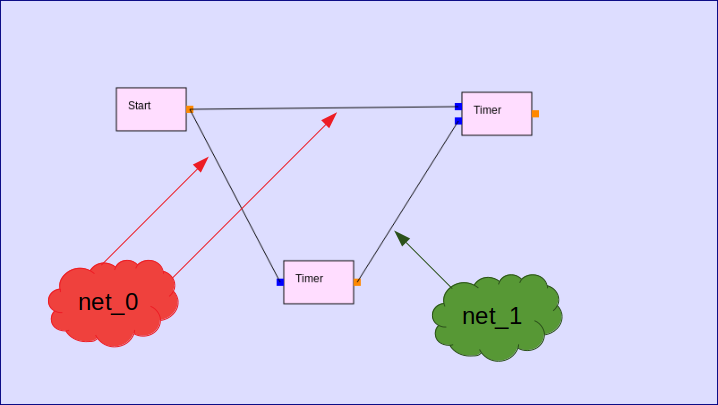
\includegraphics[width=\columnwidth]{poisson_nets.png}
    \caption{A graph representing a Poisson source with its two nets pointed out.}
    \label{fig:net}
\end{figure}

\subsubsection{Basic Info - Blue Segment}
This segment contains the most basic info about the block, namely
what type of block it is and its unique ID in the current project.

\subsubsection{Configurations - Purple Segment}
This segment contains information on how the block has been configured. Note
the similarity to associative array entries in Fig.~\ref{fig:timer_src}.

\subsubsection{Port List - Brown Segment}
This segment contains a list of all ports that are connected to a net. Every port entry contains
the port type, what mode it is operating in (some ports can operate as both inputs and outputs)
and what net the port is connected to. Ports can be connected to at most one net. Ports that
are not connected to any net do not show up here. The color coding of the net-entries correspond
to the colors of the annotations in Fig.~\ref{fig:net}.

\subsection{Syntax Check}
The DE can detect one basic error of syntactic character. This error occurs when a port is
disabled after it has had wires attached to it. This type of error is shown by the wire turning
red. The user is also alerted of this error, if it exists, when clicking the ''Syntax Check''
or ''Export'' button. This error also prevents the user from exporting the graph to an XML file.


\section{Conclusion}
A web-based DE for DMDL has been developed. It is lightweight and written in pure JS, CSS and HTML.
The interface follows a standard drag-and-drop style that is common for graphical programming
languages such as DMDL. The DE also allows the developer to export an XML that represents the graph
that defines the behaviour of the developer's protocol.

Future work include writing ''glue'' software between the exported XML-file and existing software
such as GNU Radio or LabVIEW in order to provide a backend for the DE. Another interesting topic
would be to write a custom backend for the DE that allows the protocol to be simulated in the 
web browser.

 

% An example of a floating figure using the graphicx package.
% Note that \label must occur AFTER (or within) \caption.
% For figures, \caption should occur after the \includegraphics.
% Note that IEEEtran v1.7 and later has special internal code that
% is designed to preserve the operation of \label within \caption
% even when the captionsoff option is in effect. However, because
% of issues like this, it may be the safest practice to put all your
% \label just after \caption rather than within \caption{}.
%
% Reminder: the "draftcls" or "draftclsnofoot", not "draft", class
% option should be used if it is desired that the figures are to be
% displayed while in draft mode.
%
%\begin{figure}[!t]
%\centering
%\includegraphics[width=2.5in]{myfigure}
% where an .eps filename suffix will be assumed under latex, 
% and a .pdf suffix will be assumed for pdflatex; or what has been declared
% via \DeclareGraphicsExtensions.
%\caption{Simulation results for the network.}
%\label{fig_sim}
%\end{figure}

% Note that the IEEE typically puts floats only at the top, even when this
% results in a large percentage of a column being occupied by floats.


% An example of a double column floating figure using two subfigures.
% (The subfig.sty package must be loaded for this to work.)
% The subfigure \label commands are set within each subfloat command,
% and the \label for the overall figure must come after \caption.
% \hfil is used as a separator to get equal spacing.
% Watch out that the combined width of all the subfigures on a 
% line do not exceed the text width or a line break will occur.
%
%\begin{figure*}[!t]
%\centering
%\subfloat[Case I]{\includegraphics[width=2.5in]{box}%
%\label{fig_first_case}}
%\hfil
%\subfloat[Case II]{\includegraphics[width=2.5in]{box}%
%\label{fig_second_case}}
%\caption{Simulation results for the network.}
%\label{fig_sim}
%\end{figure*}
%
% Note that often IEEE papers with subfigures do not employ subfigure
% captions (using the optional argument to \subfloat[]), but instead will
% reference/describe all of them (a), (b), etc., within the main caption.
% Be aware that for subfig.sty to generate the (a), (b), etc., subfigure
% labels, the optional argument to \subfloat must be present. If a
% subcaption is not desired, just leave its contents blank,
% e.g., \subfloat[].


% An example of a floating table. Note that, for IEEE style tables, the
% \caption command should come BEFORE the table and, given that table
% captions serve much like titles, are usually capitalized except for words
% such as a, an, and, as, at, but, by, for, in, nor, of, on, or, the, to
% and up, which are usually not capitalized unless they are the first or
% last word of the caption. Table text will default to \footnotesize as
% the IEEE normally uses this smaller font for tables.
% The \label must come after \caption as always.
%
%\begin{table}[!t]
%% increase table row spacing, adjust to taste
%\renewcommand{\arraystretch}{1.3}
% if using array.sty, it might be a good idea to tweak the value of
% \extrarowheight as needed to properly center the text within the cells
%\caption{An Example of a Table}
%\label{table_example}
%\centering
%% Some packages, such as MDW tools, offer better commands for making tables
%% than the plain LaTeX2e tabular which is used here.
%\begin{tabular}{|c||c|}
%\hline
%One & Two\\
%\hline
%Three & Four\\
%\hline
%\end{tabular}
%\end{table}


% Note that the IEEE does not put floats in the very first column
% - or typically anywhere on the first page for that matter. Also,
% in-text middle ("here") positioning is typically not used, but it
% is allowed and encouraged for Computer Society conferences (but
% not Computer Society journals). Most IEEE journals/conferences use
% top floats exclusively. 
% Note that, LaTeX2e, unlike IEEE journals/conferences, places
% footnotes above bottom floats. This can be corrected via the
% \fnbelowfloat command of the stfloats package.










% if have a single appendix:
%\appendix[Proof of the Zonklar Equations]
% or
%\appendix  % for no appendix heading
% do not use \section anymore after \appendix, only \section*
% is possibly needed

% use appendices with more than one appendix
% then use \section to start each appendix
% you must declare a \section before using any
% \subsection or using \label (\appendices by itself
% starts a section numbered zero.)
%

\if 0
    \appendices
    \section{Proof of the First Zonklar Equation}
    Appendix one text goes here.
    % you can choose not to have a title for an appendix
    % if you want by leaving the argument blank
    \section{}
    Appendix two text goes here.
\fi

% use section* for acknowledgment
\section*{Acknowledgments}
The author would like to thank Dr. Peng Wang for supervising this project, for giving valuable
feedback during the process and for sharing his work on DMDL. The author would also like to thank
Dr. Christian Schulte for providing the opportunity to carry out this project in a formal setting
and for sharing his thoughts and experiences.

% Can use something like this to put references on a page
% by themselves when using endfloat and the captionsoff option.
\newpage




% trigger a \newpage just before the given reference
% number - used to balance the columns on the last page
% adjust value as needed - may need to be readjusted if
% the document is modified later
%\IEEEtriggeratref{8}
% The "triggered" command can be changed if desired:
%\IEEEtriggercmd{\enlargethispage{-5in}}

% references section

% can use a bibliography generated by BibTeX as a .bbl file
% BibTeX documentation can be easily obtained at:
% http://mirror.ctan.org/biblio/bibtex/contrib/doc/
% The IEEEtran BibTeX style support page is at:
% http://www.michaelshell.org/tex/ieeetran/bibtex/
\bibliographystyle{IEEEtran}
% argument is your BibTeX string definitions and bibliography database(s)
\bibliography{ID2205_Leon_Fernandez_Final_Report.bib}
%
% <OR> manually copy in the resultant .bbl file
% set second argument of \begin to the number of references
% (used to reserve space for the reference number labels box)
%\begin{thebibliography}

% biography section
% 
% If you have an EPS/PDF photo (graphicx package needed) extra braces are
% needed around the contents of the optional argument to biography to prevent
% the LaTeX parser from getting confused when it sees the complicated
% \includegraphics command within an optional argument. (You could create
% your own custom macro containing the \includegraphics command to make things
% simpler here.)
%\begin{IEEEbiography}[{\includegraphics[width=1in,height=1.25in,clip,keepaspectratio]{mshell}}]{Michael Shell}
% or if you just want to reserve a space for a photo:

%\begin{IEEEbiography}{Leon Fernandez}
%Was born in 1991 and decided to become a Pokemon trainer at age 7.
%\end{IEEEbiography}


% You can push biographies down or up by placing
% a \vfill before or after them. The appropriate
% use of \vfill depends on what kind of text is
% on the last page and whether or not the columns
% are being equalized.

%\vfill

% Can be used to pull up biographies so that the bottom of the last one
% is flush with the other column.
%\enlargethispage{-5in}



% that's all folks
\end{document}


